\documentclass[colorlinks=true,pdfstartview=FitV,linkcolor=blue,
            citecolor=red,urlcolor=magenta]{ligodoc}

\usepackage{graphicx}
\usepackage{amssymb}
\usepackage{amsmath}
\usepackage{longtable}
\usepackage{rotating}
\usepackage[usenames,dvipsnames]{color}
\usepackage{fancyhdr}
\usepackage{subfigure}
\usepackage{hyperref}
\usepackage{mathtools}
\usepackage{listings}
\usepackage{minted}

\ligodccnumber{T}{17}{00198}{}{v1}% \ligodistribution{AIC, ISC}

\setlength\parindent{24pt}

\title{Online Detector Characterization using Neural Networks}

\author{Roxana Popescu}

\begin{document}

\tableofcontents

\section{Abstract}

\indent

\par Data obtained from LIGO has noise that comes from many sources. To be able to better distinguish signals from the noise, it is important to characterize the type of noise observed. Machine learning algorithms can be used to look for patterns within the data and to classify the data into distinct categories. We are using clustering algorithms, such as kmeans, to identify earthquakes in seismic noise data. To test how well the clustering algorithms work, we compare the clusters to the times when earthquake waves reach the detector site. This comparison will be used to evaluate how well a neural network determines earthquakes compared to the clustering algorithms.

\section{Introduction} 

\indent

\par The data obained from LIGO contains noise that comes from many sources. In order to be able to better distinguish signals from the noise, it is important to characterize the type of noise observed. Machine learning algorithms can be used to look for patterns within the data and to classify or cluster the data into different categories.

\par There are many sensors near the LIGO detectors that measure sources of noise. For example, there are several stations at each LIGO detector that measure seismic noise in different frequency channels in each of the X,Y, and Z directions. Within the data, there are different types of seismic noise such as earthquakes and anthropogenic noise.  

\par In order to sort data, machine learning algorithms can use one of two approaches: classification or clustering. Classification algorithms search the data and sort the data into already defined categories. Clustering algorithms look for relationships within the data to create categories into which the data is then sorted. Classification algorithms are part of supervised learning since the computer determines the structure of the data from data that is already provided. Clustering algorithms are part of unsupervised learning since the computer determines the structure of the data without any previous information. Clustering algorithms can be used to characterize the noise by identifying common characteristics within the noise and the clustering algorithms can further help with classification. \cite{Citation1}

\par Neural networks can be used to find relationships between the inputed data by using hidden layers of connections within the data. Neural networks consist of layers of units called artifical neurons, which activate based on whether inputs into the unit meet a certain threshold. \cite{Citation1}

\par The aim of this project was to characterize different sources of noise from LIGO using machine learning algorithms. First we tested clustering algorithms on seismic data, and then implemented a neural network to characterize the seismic noise data.

\section{Clustering Algorithms}

\subsection{K-means Clustering}

\indent

\par The k-means clustering algorithm creates clusters by separating data points into k number of groups. The value of k is inputted into the algorithm. The clusters are determined by minimizing the inertia, or the within-cluster sum-of-squares. The inertia is a measure of how coherent the clusters are. By minimizing the intertia, the algorithm tries to minimize the difference between the mean value of a cluster and the values of points in the cluster. If a set of n samples x are inputted, the algorithm divides the samples into k clusters that are referred to as  C. Each cluster is described by its mean \(u_j\), or centroid. The interia of a cluster is caluclated by the following expression:

\[\sum_{i=0}^{n} \min_{\mu_j \in  C}(\|x_j-\mu_i\|^2)\]

\par The inertia is not normalized, but lower values are better and zero is the optimum value. The inertia assumes that the clusters are convex and isotropic, and would not work well to cluster irregular or elongated clusters. \cite{Citation2}\cite{Citation3} 

\subsection{DBSCAN Clustering}

\indent

\par The DBSCAN clustering algorithm creates clusters out of areas in the data of higher density. Unlike kmeans, it does not consider clusters to have any particular shapes, and the algorithm determines the number of clusters based on inputted parameters. Core samples are points that are in areas of high densities. The algorithm creates clusters around core samples so that the clusters consist of core samples, and non-core samples that are close to the core samples. The core samples are determined by two input parameters, the minimum samples and a specified distance, $\varepsilon$. A point is in the $\varepsilon$-neighborhood if the distance d from a point p to a point q is within a radius of of $\varepsilon$. High density areas have the minimum sample of values within the $\varepsilon$-neighborhood. By increasing the number of minimum samples, and decreasing the distance, $\varepsilon$, a cluster's density is increased. \cite{Citation2}\cite{Citation4}

\subsection{Agglomerative Clustering}

\indent

\par Agglomerative clustering is a type of hierarchical clustering algorithm. Hierarchical clustering builds clusters by merging and splitting clusters many times. Agglomerative clustering works by initially giving each data point its own cluster and then merging the clusters until the inputed number of clusters is reached. \cite{Citation2}

\subsection{Birch Clustering}

\indent

\par Birch clustering stands for balanced iterative reducing and clustering hierarchies. It is a hierarchical clustering algorithm which builds clusterings by merging and splitting clusters many times. \cite{Citation5}

\subsection{Evaluating Clustering Algorithms}

\subsubsection{Calinsky Harabaz Index}

\indent

\par The Calinsky-Harabaz index is a method used to evaluate how well clustering algorithms work, that does not require input of external data. The Calinsky-Harabaz score is calculated by finding the ratio of the between-clusters dispersion mean to the within-cluster dispersion mean. This ratio is calculated as follows:

\[s(k) = \frac{Tr(B_k)}{Tr(W_k)}\times\frac{N-k}{k-1}\]

\par Where k is the number of clusters, \(B_k\) is the between group dispersion matrix, \(W_k\) is the within group dispersion matrix and N is the number of data points. \(W_k\) and  \(B_k\) are defined by:

\[W_k = \sum_{q=1}^{k} \sum_{x \in C_q} (x-c_q)(x-c_q)^T\]

\[B_k = \sum_{q} n_q (c_q-c)(c_q-c)^T\]

\par Where \(C_q\) is the number of set points in cluster q, \(c_q\) is the center of cluster q, c is the center of the clusters, and \(n_q\) is the number of points in cluster q. \cite{Citation2} 

\subsubsection{Comparing Clusters to Earthquake Times}

\indent 

\par Another way to evaluate how well the clustering algorithms work is to add up the cluster labels that occur five  minutes before and after an earthquake Rayleigh wave arrives, to add up the total amount of cluster labels, and for each individual cluster to divide the number of cluster labels that appear near the earthquake by the total number of cluster labels. For each cluster k, the earthquake comparison score, E(k) can be determined by:

\[E(k) = \frac{N_e}{N_t}\]

Where \(N_e\) is the number of cluster labels five minutes before and after an earthquake, and \(N_t\) is the total number of cluster labels. If a cluster corresponds to the presence of an earthquake then it will have a high percentage of its cluster labels present near an earthquake.  

\section{Clustering Results}

\indent

\par I compared how well the clusters determined by clustering algorithms correspond to earthquakes that show up as peaks in the data. I read in seismic data taken from three seismometers. I read in the earthquake band channels from the data and then clustered the channels using kmeans, and dbscan. The script counts the cluster labels five mintues before and after the time when earthquake Rayleigh waves arrive at the site as well as the total number of cluster labels. For each individual cluster, the earthquake comparison score is calculated. Only earthquakes with ground displacement greater than 65 percentile are considered. This score is used to determine how well a cluster corresponds to an earthquake. 

\par I have used seismic data from the Hanford observatory from March 2017. I have clustered the data from the earthquake channels using kmeans, and  dbscan. I've also used the Calinsky-Harabaz index to evaluate how well the clustering works. Tables \ref{Table 1} and \ref{Table 2} show the clustering results for the kmeans and dbscan algorithms respectively.

\begin{table}[h!]
\centering
 \begin{tabular}{| m{3.5cm} m{3.5cm} m{3.5cm} m{3.5cm}|} 
 \hline
 Number of Clusters & Calinsky-Harabaz Score & Cluster of Earthquake Score & Earthquake Score\\ [0.5ex] 
 \hline\hline
 2 & 40192 & 1 & 0.5\\ 
 \hline
 3 & 37288 & 1 & 0.48\\
 \hline
 4 & 43960 & 2 & 0.31\\
 \hline
 5 & 44225 & 2 & 0.34\\
 \hline
 6 & 45618 & 2 & 0.33\\ 
 \hline
 7 & 46338 & 2 & 0.33\\
 \hline
 8 & 46349 & 1 & 0.44\\
 \hline
 9 & 46190 & 3 & 0.59\\
 \hline
 10 & 45323 & 6 & 0.75\\
 \hline
 Average & 43943 & N/A & 0.45\\
 \hline
 \end{tabular}
 \caption{Results of kmeans clustering}
 \label{Table 1}
\end{table}

\begin{table}[h!]
\centering
 \begin{tabular}{|m{2cm} m{2.25cm} m{2.25cm} m{2.25cm} m{2.25cm} m{2.25cm}|} 
 \hline
 Epsilon Value & Minimum Samples & Number of Clusters & Calinsky-Harabaz Score & Cluster of Earthquake Score & Earthquake Score\\ [0.5ex] 
 \hline\hline
 1 & 15 & 1 & 14 & -1 & 0.01\\ 
 \hline
 2 & 10 & 15  & 5 & -1 & 0.01\\
 \hline
 2 & 15 & 5 & 6 & -1 & 0.01\\ 
 \hline
 2 & 20 & 1 & 14 & -1 & 0.01\\
 \hline
 2 & 25 & 1 & 14 & -1 & 0.01\\
 \hline
 2 & 30 & 1 & 14 & -1 & 0.01\\
 \hline
 3 & 15 & 6 & 123 & -1 & 0.01\\
 \hline
 4 & 15 & 8 & 194 & -1 & 0.01\\
 \hline
 \end{tabular}
 \caption{Results of DBSCAN clustering}
 \label{Table 2}
\end{table}

\par The dbscan clustering algorithm does not seem to work well because it places the majority of its points in the noise cluster (indicated as -1)  which results in most of the points near earthquakes being classified as noise.

\par A plot of the data clustered by kmeans is shown in Figure \ref{fig:image1} and Figure \ref{fig:image2}. The lines that indicate the time that the Rayleigh waves from the earthquake reach the sight do not align with the peaks of the earthquakes on the plot. As a result, a new criteria was defined to evaluate how well the clusters align with earthquake predictions. The peaks in the data are taken to be earthquakes and the peak earthquake score  counts the cluster labels five mintues before and after the center of the ppeaks. This score is used to determine how well a cluster corresponds to an earthquake as determined from peaks in the data. Tables \ref{Table 3}, \ref{Table 4}, \ref{Table 5}, and \ref{Table 6} show the clustering results for the kmeans, dbscan, agglomerative clustering, and birch algorithms, respectively.A plot of the data clustered by kmeans, and compared with peaks in the data, is shown in Figure \ref{fig:image3} and Figure \ref{fig:image4}.

\begin{table}[h!]
\centering
 \begin{tabular}{| m{3.5cm} m{3.5cm} m{3.5cm} m{3.5cm}|} 
 \hline
 Number of Clusters & Calinsky-Harabaz Score & Cluster of Earthquake Score & Earthquake Score\\ [0.5ex] 
 \hline\hline 
 2 & 40172 & 1 & 0.03\\ 
 \hline
 3 & 37282 & 1 & 0.04\\
 \hline
 4 & 43960 & 1 & 0.07\\
 \hline
 5 & 44225 & 4 & 0.08\\
 \hline
 6 & 45616 & 3 & 0.08\\ 
 \hline
 7 & 46338 & 3 & 0.08\\
 \hline
 8 & 46349 & 7 & 0.11\\
 \hline
 9 & 46095 & 1 & 0.11\\
 \hline
 10 & 46747 & 6 & 0.13\\
 \hline
 Average & 46747 & N/A & 0.08\\
 \hline
 \end{tabular}
 \caption{Results of kmeans clustering (Earthquake score determined by peaks)}
 \label{Table 3}
\end{table}

\begin{table}[h!]
\centering
 \begin{tabular}{|m{2cm} m{2.25cm} m{2.25cm} m{2.25cm} m{2.25cm} m{2.25cm}|} 
 \hline
 Epsilon Value & Minimum Samples & Number of Clusters & Calinsky-Harabaz Score & Cluster of Earthquake Score & Earthquake Score\\ [0.5ex] 
 \hline\hline
 1 & 15 & 1 & 14 & -1 & 0.0125\\ 
 \hline
 2 & 10 & 15  & 5 & -1 & 0.0126\\
 \hline
 2 & 15 & 5 & 6 & -1 & 0.0125\\ 
 \hline
 2 & 20 & 1 & 14 & -1 & 0.0125\\
 \hline
 2 & 25 & 1 & 14 & -1 & 0.0125\\
 \hline
 2 & 30 & 1 & 14 & -1 & 0.0125\\
 \hline
 3 & 15 & 6 & 123 & -1 & 0.0141\\
 \hline
 4 & 15 & 6 & 194 & -1 & 0.0159\\
 \hline
 5 & 15 & 8 & 373 & -1 & 0.0176\\
 \hline
 \end{tabular}
 \caption{Results of DBSCAN clustering (Earthquake score determined by peaks)}
 \label{Table 4}
\end{table}

\begin{table}[h!]
\centering
 \begin{tabular}{| m{3.5cm} m{3.5cm} m{3.5cm} m{3.5cm}|} 
 \hline
 Number of Clusters & Calinsky-Harabaz Score & Cluster of Earthquake Score & Earthquake Score\\ [0.5ex] 
 \hline\hline
 2 & 37801 & 1 & 0.04\\ 
 \hline
 3 & 33282 & 0 & 0.04\\
 \hline
 4 & 40010 & 1 & 0.08\\
 \hline
 5 & 40007 & 1 & 0.08\\
 \hline
 6 & 40339 & 1 & 0.08\\ 
 \hline
 7 & 43396 & 0 & 0.08\\
 \hline
 8 & 42621 & 3 & 0.13\\
 \hline
 9 & 42045 & 8 & 0.13\\
 \hline
 10 & 41586 & 8 & 0.13\\
 \hline
 Average & 46747 & N/A & 0.08\\
 \hline
 \end{tabular}
 \caption{Results of agglomerative clustering (Earthquake score determined by peaks)}
 \label{Table 5}
\end{table}

\begin{table}[h!]
\centering
 \begin{tabular}{| m{3.5cm} m{3.5cm} m{3.5cm} m{3.5cm}|} 
 \hline
 Number of Clusters & Calinsky-Harabaz Score & Cluster of Earthquake Score & Earthquake Score\\ [0.5ex] 
 \hline\hline
 2 & 37801 & 1 & 0.04\\ 
 \hline
 3 & 33282 & 0 & 0.04\\
 \hline
 4 & 40010 & 1 & 0.08\\
 \hline
 5 & 40007 & 1 & 0.08\\
 \hline
 6 & 40339 & 1 & 0.08\\ 
 \hline
 7 & 43396 & 0 & 0.08\\
 \hline
 8 & 42621 & 3 & 0.13\\
 \hline
 9 & 42045 & 8 & 0.13\\
 \hline
 10 & 41586 & 8 & 0.13\\
 \hline
 Average & 46747 & N/A & 0.08\\
 \hline
 \end{tabular}
 \caption{Results of birch clustering (Earthquake score determined by peaks)}
 \label{Table 6}
\end{table}

\par Based on the earthquake score based on peaks, the kmeans clustering algorithm does not appear to agree very well with results.  The agglomerative clustering and birch clustering algorithms give the same results, which are not very different from the kmeans clustering results. None of the clustering algorithms have clusters that clearly identify earthquakes.  

\par In order to obtain clusters that better correspond to earthquakes, I added rows to the data that are shifted by time and inputted this timeshifted data into the clustering algorithms. Table \ref{Table 7} shows the average comarpison of different timeshifts for the kmeans clustering algorithm. 

\begin{table}[h!]
\centering
 \begin{tabular}{| m{4cm} m{4cm} m{4cm}|} 
 \hline
 Timeshift (minutes) & Calinsky-Harabaz Average & Maximum Earthquake Score Average\\ [0.5ex] 
 \hline\hline
 0 & 44087 & 0.08\\
 \hline
 10 & 49251 & 0.08\\
 \hline
 30 & 44081 & 0.09\\
 \hline
 60 & 44066 & 0.08\\
 \hline
 \end{tabular}
 \caption{Results of Timeshifted Kmeans Clustering (Earthquake score determined by peaks)}
 \label{Table 7}
\end{table}

\par Shifting the data and applying the kmeans clustering algorithm does not improve the performance of the kmeans clustering algorithm.  

\section{Neural Network Results}

\indent

\par The neural network was implemented using the keras package with tensforflow as a backend. Earthquake channel seismic BLRMS data from Hanford during March 2017 was timeshifted by 30 mintues and then read into the neural network. For each point in the data it was indicated whether or not it corresponds to an earthquake. The peaks in the data were used to determine which points correspond to eartquakes. Points that occur 5 minutes before and after a peak in the data. The neural network consists of a sequential model with three dense layers.

\par An accuracy of 0.998 is obtained when using part of the data set to validate the trained neural network. A plot of the neural network is shown in figures \ref{image:fig5} and  \ref{image:fig6}. The vertical lines correspond to peaks in data that are caused by earthquakes. The dotted lines indicate where the neural network detects an earthquake. The neural network does a better job of detecting earthquakes than the clustering algorithms based on comparing how well the neural network detects earthquakes to how the clustering algorithm detects earthquakes. However, more data is needed in order to test the neural network, and to improve the accuray of the neural network. 

\section{Acknowledgments}

\indent

\par I would like to thank the LIGO SURF Program as well as  Dr. Rana Adhikari, Dr. TJ Massinger, and Dr. Jess McIver for help and guidance in this project.

\begin{figure}[htbp]
\begin{center}
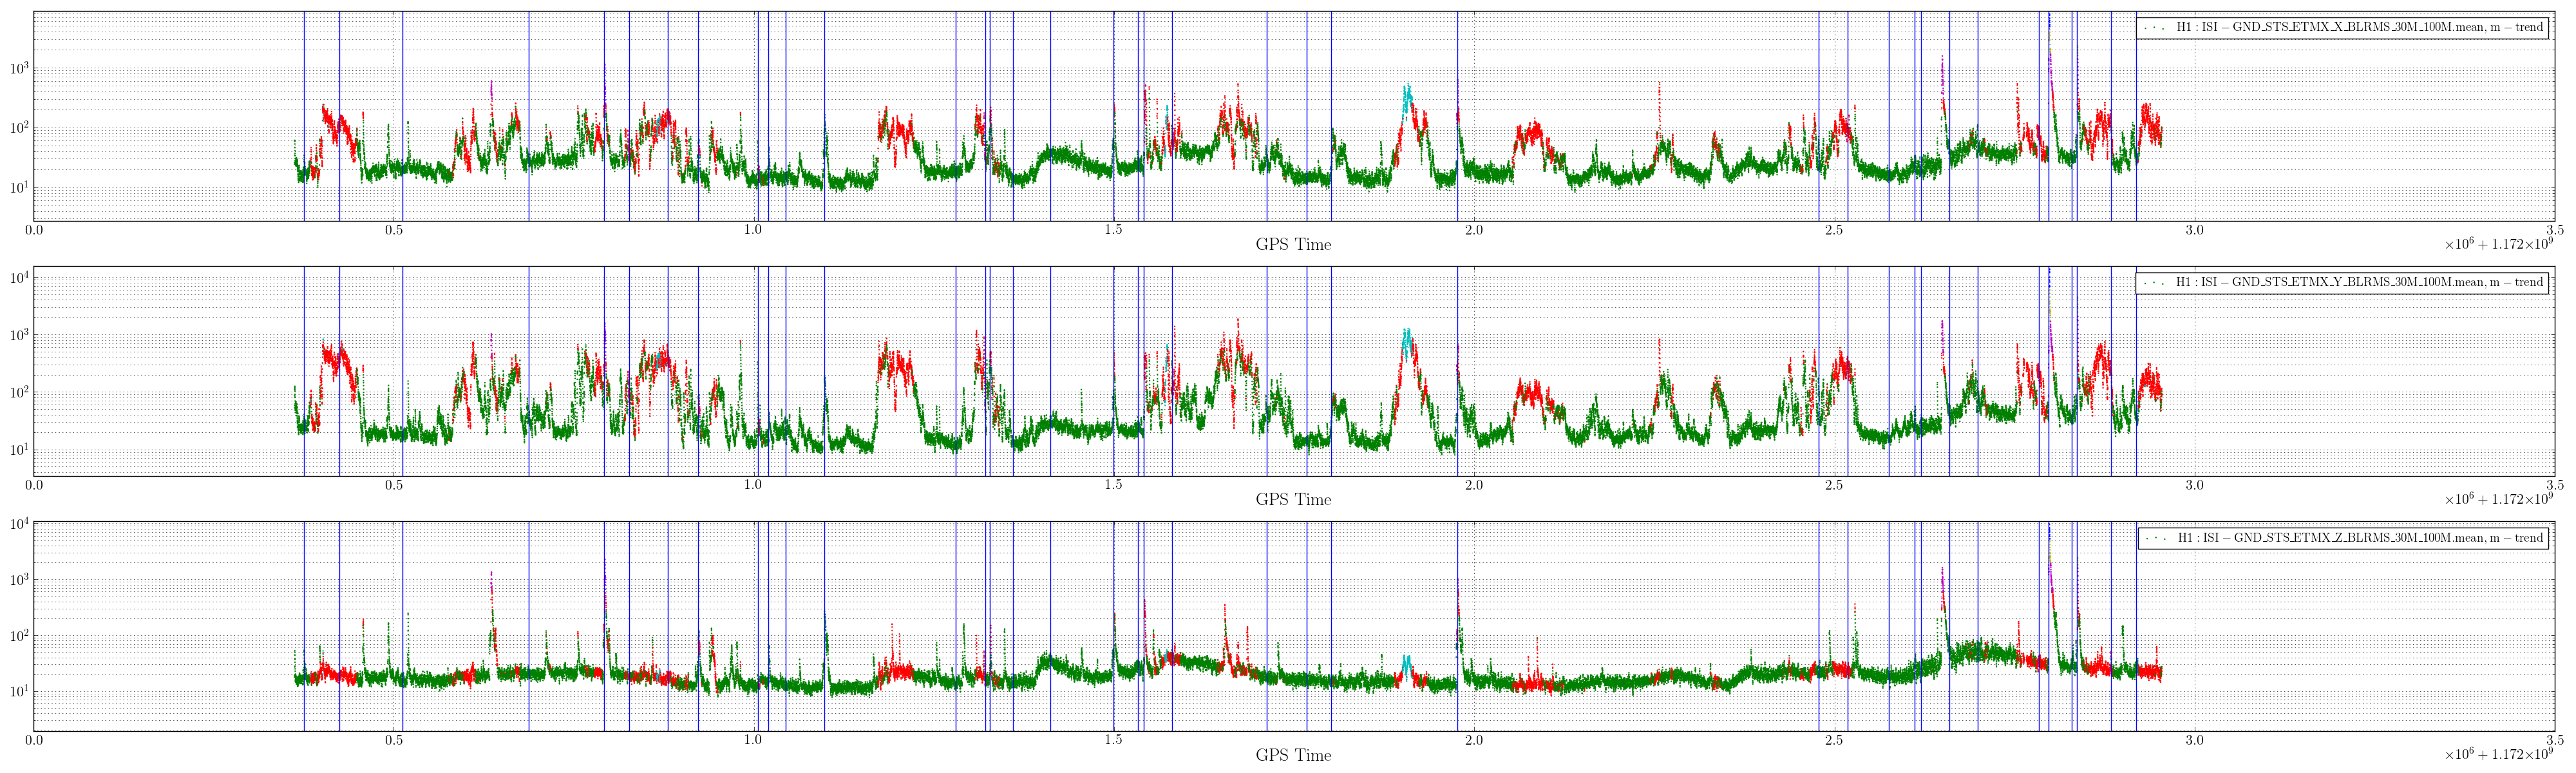
\includegraphics[width=1.3\textwidth,angle=90]{EQdata_Kmeans_6_.png}
\caption{Plot of data from earthquake channels clustered using kmeans with k=6 (earthquakes indicated)}
\label{fig:image1}
\end{center}
\end{figure}

\begin{figure}[htbp]
\begin{center}
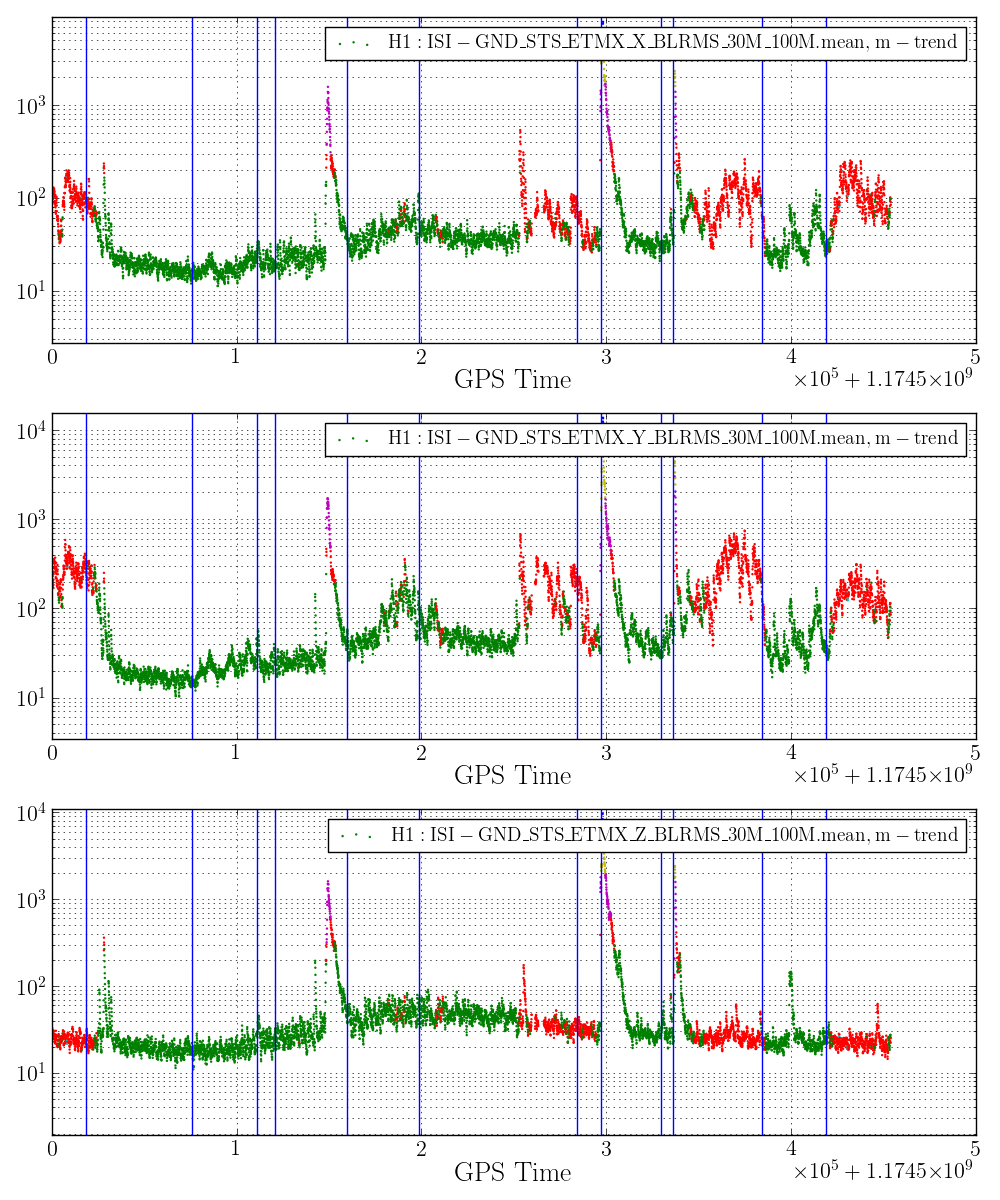
\includegraphics[scale = 0.5]{EQdata2_Kmeans_6_crop.png}
\caption{Figure 1 zoomed in for detail}
\label{fig:image2}
\end{center}
\end{figure}

\begin{figure}[htbp]
\begin{center}
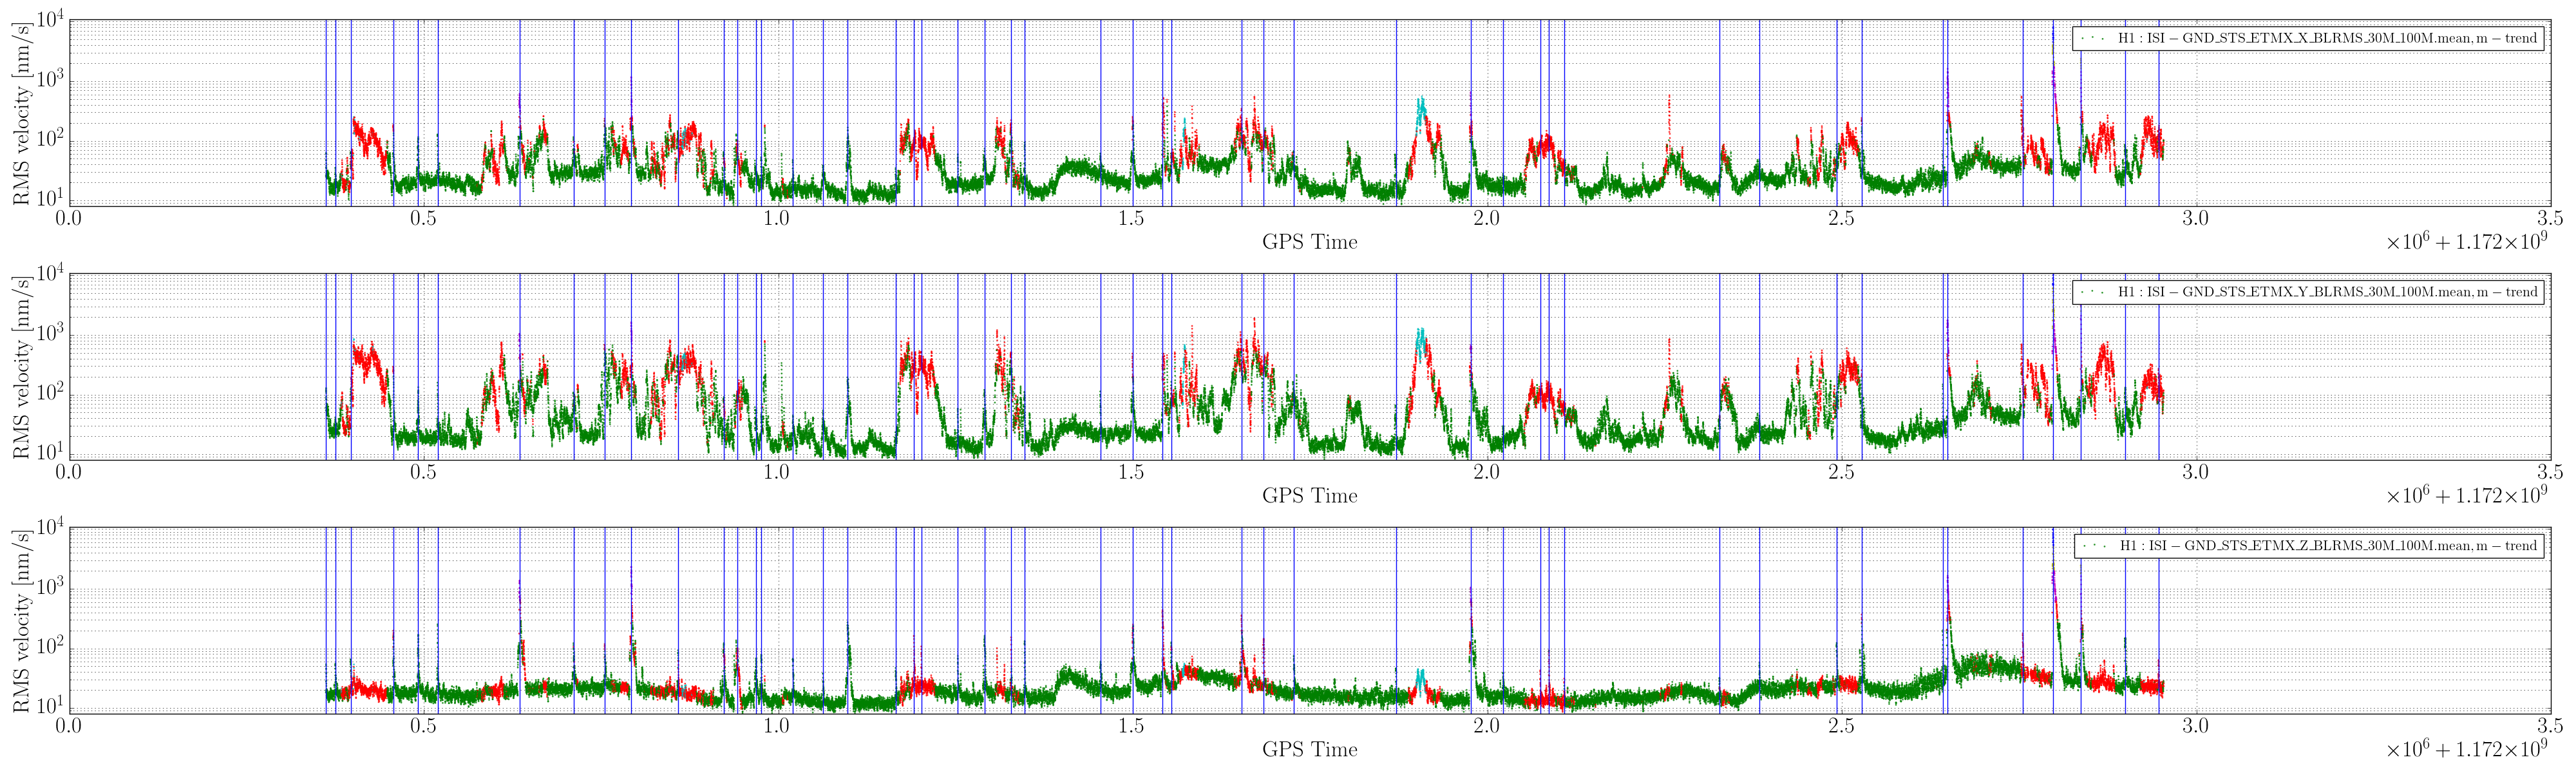
\includegraphics[width=1.3\textwidth,angle=90]{EQdata_Kmeans_6_2.png}
\caption{Plot of data from earthquake channels clustered using kmeans with k=6 (peaks indicated)}
\label{fig:image3}
\end{center}
\end{figure}

\begin{figure}[htbp]
\begin{center}
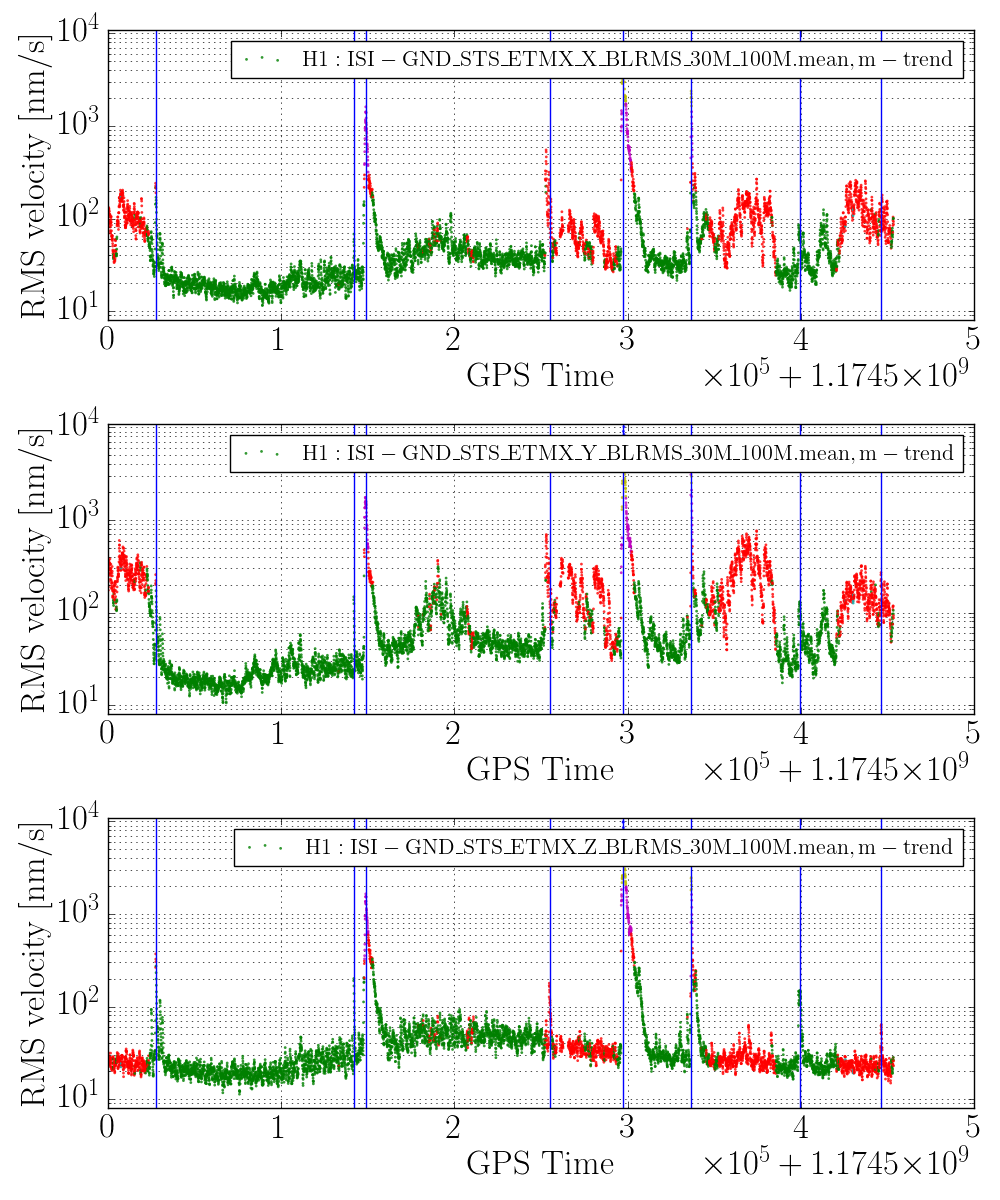
\includegraphics[scale = 0.5]{EQdata_Kmeans_6_crop_2.png}
\caption{Figure 3 zoomed in for detail}
\label{fig:image4}
\end{center}
\end{figure}

\begin{figure}[htbp]
\begin{center}
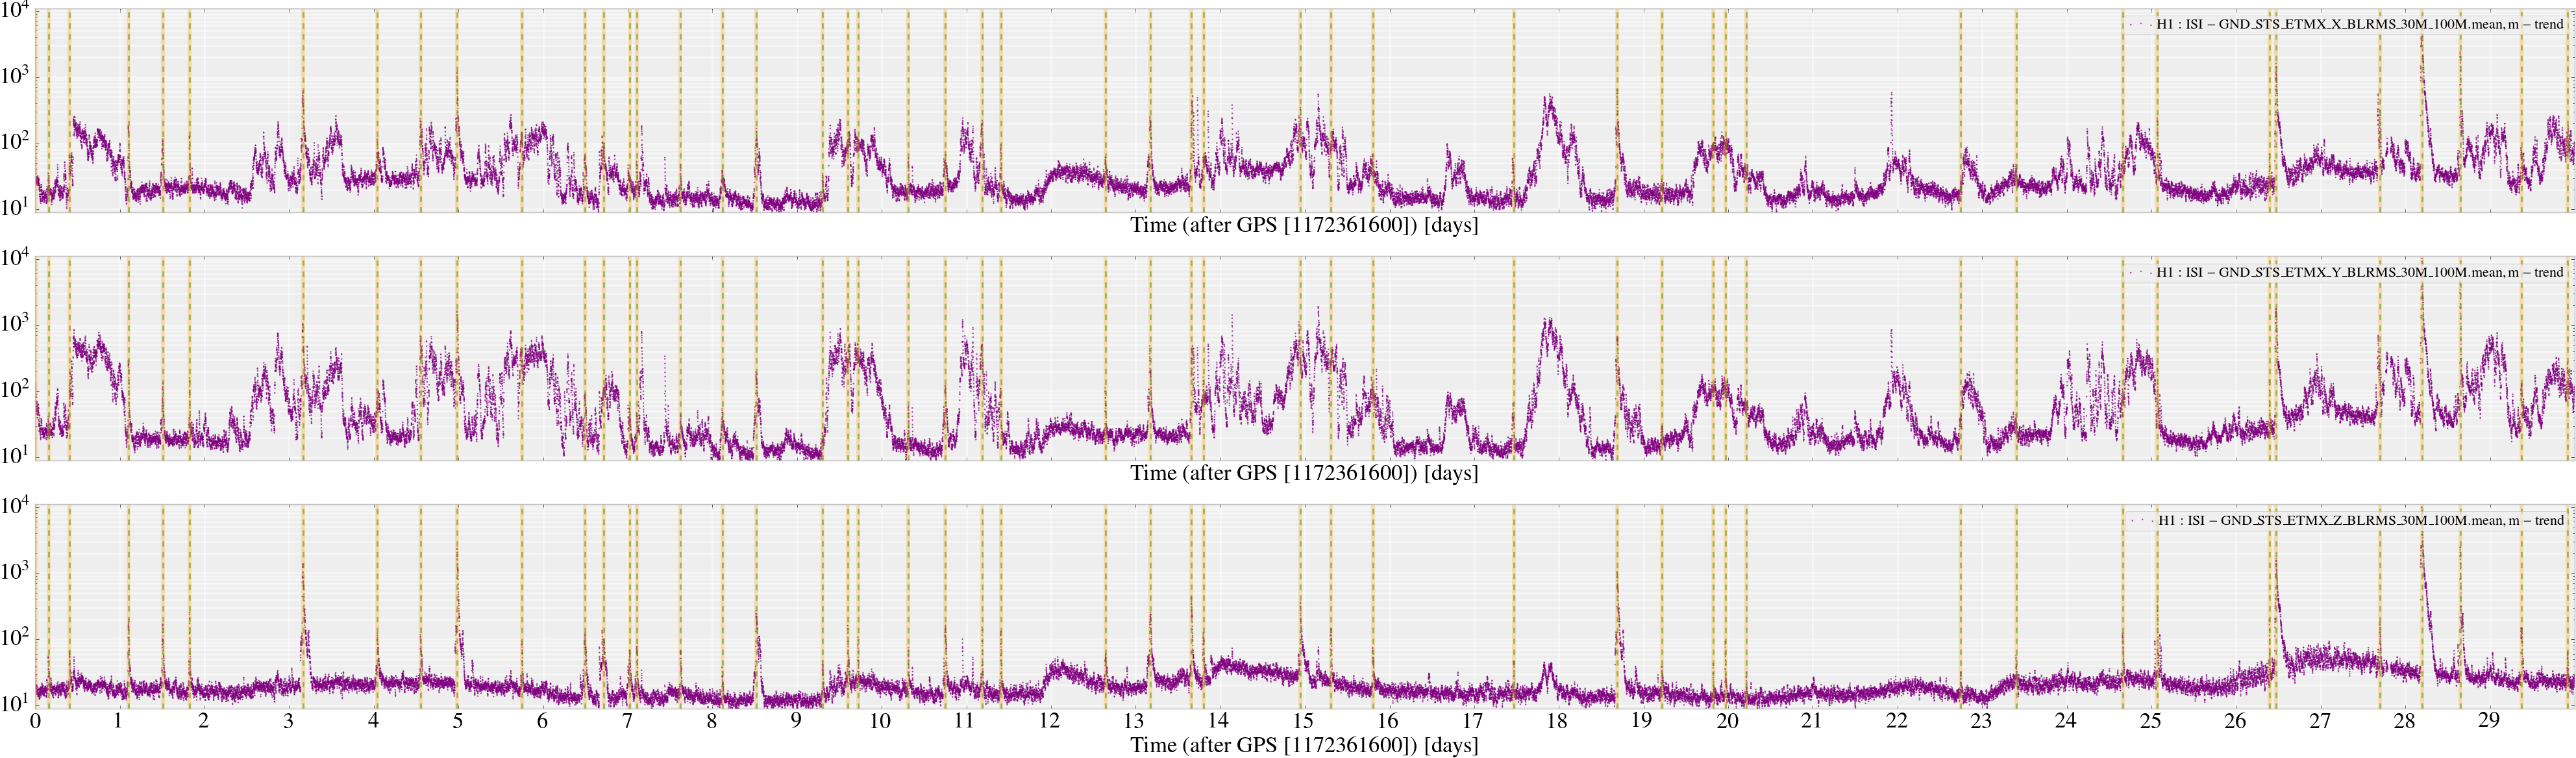
\includegraphics[width=1.3\textwidth,angle=90]{ConvNet-Comparison2.png}
\caption{Plot of data from earthquake channels classified by neural net (peaks indicated)}
\label{fig:image5}
\end{center}
\end{figure}

\begin{figure}[htbp]
\begin{center}
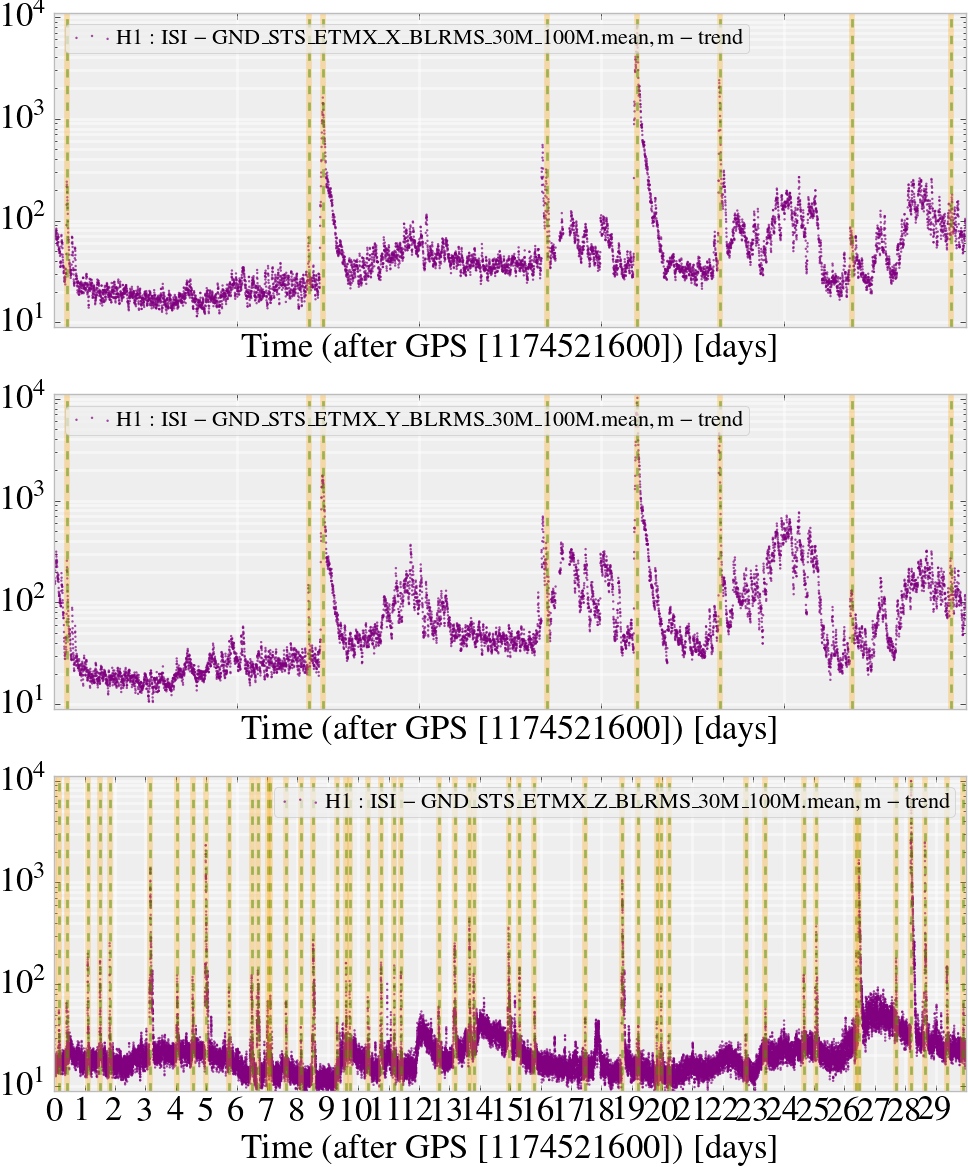
\includegraphics[scale = 0.35]{ConvNet-Comparison2_crop.png}
\caption{Figure 6 zoomed in for detail}
\label{fig:image6}
\end{center}
\end{figure}

\begin{thebibliography}{9}
      
	\bibitem{Citation1}
	  Aurelien Geron,
	  \emph{Hands-On Machine Learning with Scikit-Learn and TensorFlow}.
	  O'Reilly Media Inc., (2017).    
        
        \bibitem{Citation2}
          \url{http://scikit-learn.org/stable/modules/clustering.html}

        \bibitem{Citation3}
          David Arthur, Sergei Vassilvitskii,
          \emph{k-means++: The Advantages of Careful Seeding}.
          Proceedings of the Eighteenth Annual ACM-SIAM Symposium on Discrete Algorithms, Society of Industrial and Applied Mathematics, (2007).

        \bibitem{Citation4}
          Martin Ester, Hans-Peter Kriegel, Jorg Sander, Xiaowei Xu,
          \emph{A Density-Based Algorithm for Discovering Clusters in Large Spatial Databases with Noise}.
          Proceedings of the 2nd International Conference on Knowledge Discovery and Data Mining, (1996).

        \bibitem{Citation5}
          Tian Zhang, Raghu Ramakrishnan, Miron Liviny
          \emph{BIRCH: An Efficient Data Clustering Method for Very Large Databases}
          Proceedings of the 1996 ACM SIGMOD international conference on Management of data, (1996). 
          
\end{thebibliography}

\appendix
\section{Script for Evaluating Clustering Algorithms}
\begin{minted}{python}
'''
This script reads in seismic noise data from March 2017 and earthquake data.
It shifts the data by time for clustering
It determined earthquake times by looking at peaks in data
It clusters earthquake channels using kmeans and dbscan.
It compares the clusters around the earthquake times to deterime effectiveness of clustering
It plots the data as clustered by kmeans and dbscan
'''

from __future__ import division
from sklearn.cluster import KMeans
from sklearn.cluster import DBSCAN
from sklearn.cluster import AffinityPropagation
from sklearn.cluster import MeanShift,estimate_bandwidth
from sklearn.cluster import spectral_clustering
from sklearn.cluster import AgglomerativeClustering
from sklearn.cluster import Birch
from sklearn import metrics
from sklearn.preprocessing import StandardScaler
import numpy as np
from scipy.io import loadmat
import matplotlib
matplotlib.use('Agg')
import matplotlib.pyplot as plt
from matplotlib.pyplot import cm
import scipy.signal as sig
from astropy.time import Time
import collections

plt.rc('text',   usetex = True)
plt.rc('font',   **{'family': 'serif', 'serif': ['Computer Modern']})
plt.rc('axes',   labelsize = 20.0)
plt.rc('axes',   axisbelow = True)
plt.rc('axes.formatter', limits=[-3,4])
plt.rc('legend', fontsize  = 14.0)
plt.rc('xtick',  labelsize = 16.0)
plt.rc('ytick',  labelsize = 16.0)
plt.rc('figure', dpi = 100)

# colors for clusters
colors = np.array(['r', 'g', 'b','y','c','m','darkgreen','plum',
                       'darkblue','pink','orangered','indigo'])
cl          = 6   # number of clusters for kmeans
eps         = 2   # min distance for density for DBscan
min_samples = 15  # min samples for DBscan

#read in data
H1dat = loadmat('Data/' + 'H1_SeismicBLRMS.mat')
#edat  = np.loadtxt('Data/H1_earthquakes.txt')

# read in earthquake channels
cols   = [6,12,18,24,30,36,42,48]      # NEED comment here
vdat   = np.array(H1dat['data'][0])
vchans = np.array(H1dat['chans'][0])
for i in cols:
    add = np.array(H1dat['data'][i])
    vdat = np.vstack((vdat, add))
for i in cols:
    vchans = np.append(vchans,H1dat['chans'][i])
timetuples = vdat.T

# shift the data
vdat2   = vdat
vchans2 = vchans
num     = 10
t_shift = 10 # how many minutes to shift the data by
for i in cols:
    add = np.array(H1dat['data'][i])
    for j in range(1, t_shift+1):
        add_shift = add[j:]
        add_values = np.zeros((j,1))
        add_shift = np.append(add_shift, add_values)
        vdat2 = np.vstack((vdat2, add_shift))
        chan = 'Time_Shift_' + str(j) + '_Min_EQ_Band_' + str(i)
        vchans2 = np.append(vchans2, chan)
print(np.shape(vdat2))
vdat2 = vdat[:,:43200-t_shift]
print(np.shape(vdat2))
timetuples2 = vdat.T
timetuples3 = vdat[0:num].T

 #convert time to gps time
times       = '2017-03-01 00:00:00'
ti           = Time(times,format='iso',scale='utc')
t_start     = int(np.floor(ti.gps/60)*60)
dur_in_days = 30
dur_in_minutes = dur_in_days*24*60
dur         = dur_in_minutes*60
t_end       = t_start + dur
t    = np.arange(t_start, t_end, 60)

# create list of earthquake times from peaks
# find peaks in all three z channel directions
widths  = np.arange(5, 140)   # range of widths in minutes
min_snr = 5
noise_perc = 15
peaks1 = sig.find_peaks_cwt(vdat[2], widths,
                                min_snr = min_snr, noise_perc=noise_perc)
peaks2 = sig.find_peaks_cwt(vdat[5], widths,
                                min_snr = min_snr, noise_perc=noise_perc)
peaks3 = sig.find_peaks_cwt(vdat[8], widths,
                                min_snr = min_snr, noise_perc=noise_perc)

# takes average time for earthquake times from three channels
# that are within dtau minutes of each other 
dtau = 3
peak_list = np.array([])
for i in peaks1:
    for j in peaks2:
        for k in peaks3:
            if (abs(i-j) <= dtau and abs(i-k) <= dtau):
                avg = (i+j+k)/3
                peak_list = np.append(peak_list, avg)
EQ_times = np.array([])
for i in peak_list:
    EQ_times = np.append(EQ_times, t[int(i)])

# kmeans clustering loop

Nmin = 2
num = 9
Nmax = Nmin + num  
for cl in range(Nmin, Nmax):
    kmeans   = KMeans(n_clusters=cl, random_state=13).fit(timetuples2)
    kpoints  = np.array([])
    xvals    = np.arange(t_start, t_end, 60)
    for t in EQ_times: #for each EQ: collect indices within 30 min of EQ
        tmin = int(t - 10)
        tmax = int(t + 10)
        for j  in range(tmin, tmax):
            val     = abs(xvals - j)
            aval    = np.argmin(val)
            kpoints = np.append(kpoints, aval)
    kpoints   = np.unique(kpoints) # make sure there are no repeating indices
    kclusters = np.array([])
    for i in kpoints:
        #for each index find the corresponding cluster and store them in array
        kclusters = np.append(kclusters, kmeans.labels_[int(i)])
        # kmeans score determined by ratio of points in
        # cluster/points near EQ to  points in cluster/all points
    k_count      = collections.Counter(kclusters).most_common()
    ktot_count   = collections.Counter(kmeans.labels_).most_common()
    k_list_cl    = [x[0] for x in k_count] #cluster number
    k_list       = [x[1] for x in k_count] #occurences of cluster
    ktot_list_cl = [x[0] for x in ktot_count]
    ktot_list    = [x[1] for x in ktot_count]
    k_clusters   = np.array([])
    k_compare    = np.array([])
    k_list2      = np.array([])
    ktot_list2   = np.array([])
    # arrange so that k_clusters k_list2 and k_compare are in the same order
    for i in range(len(k_list_cl)):
        for j in range(len(ktot_list_cl)):
            if k_list_cl[i] == ktot_list_cl[j]:
                k_clusters = np.append(k_clusters,k_list_cl[i])
                compare    = k_list[i]/ktot_list[j]
                k_compare  = np.append(k_compare, compare)
                k_list2    = np.append(k_list2, k_list[i])
                ktot_list2 = np.append(ktot_list2, k_list[i])
    np.set_printoptions(precision=3)
    #print(k_clusters)
    #print(k_compare)
    max_val = max(k_compare)
    max_index = np.argmax(k_compare)
    max_cluster = int(k_clusters[max_index])
    k_cal_score = metrics.calinski_harabaz_score(timetuples, kmeans.labels_)
    #print('K-means ' + str(cl) + ':  C-H score = {:0.6g}'.format(k_cal_score))
    print(str(cl) + ' & {:0.6g}'.format(k_cal_score) + ' & ' + str(max_cluster) + ' & {:0.6g}'.format(max_val))
    print('\\hline')


# dbscan clustering loop

min_samples_list = [10,20,25,30]
eps_list  = [1,2,3,4,5]
#for min_samples in min_samples_list:
for eps in eps_list:
    db = DBSCAN(eps=eps,min_samples=min_samples).fit(timetuples)
    #number of clusters
    n_clusters = len(set(db.labels_)) - (1 if -1 in db.labels_ else 0)
    #add up number of clusters that appear next to each earthquake
    xvals = np.arange(t_start,t_end,60)
    dbpoints = np.array([])
    for t in EQ_times: #for each EQ: collect indices within 5 min of EQ
        tmin = int(t-5*60)
        tmax = int(t+5*60)
        for j  in range(tmin,tmax):
            val = abs(xvals-j)
            aval = np.argmin(val)
            dbpoints  = np.append(dbpoints, aval)
    dbpoints = np.unique(dbpoints)
    dbclusters = np.array([])
    for i in dbpoints: dbclusters = np.append(dbclusters,db.labels_[int(i)]) #for each index find the corresponding cluster and store them in array
    #dbscan score determined by percent of points sorted into one cluster near EQ
    db_count = collections.Counter(dbclusters).most_common()
    dbtot_count = collections.Counter(db.labels_).most_common()
    db_list_cl = [x[0] for x in db_count]
    db_list = [x[1] for x in db_count]
    dbtot_list_cl = [x[0] for x in dbtot_count]
    dbtot_list = [x[1] for x in dbtot_count]
    db_clusters = np.array([])
    db_compare = np.array([])
    db_list2 = np.array([])
    dbtot_list2 = np.array([])
    for i in range(len(db_list_cl)):
        for j in range(len(dbtot_list_cl)):
            if db_list_cl[i] == dbtot_list_cl[j]:
                db_clusters = np.append(db_clusters,db_list_cl[i])
                compare = db_list[i]/dbtot_list[j]
                db_compare = np.append(db_compare, compare)
                db_list2 = np.append(db_list2, db_list[i])
                dbtot_list2 = np.append(dbtot_list2, db_list[i])
    #print(db_clusters)
    #print(db_compare)
    max_val = max(db_compare)
    max_index = np.argmax(db_compare)
    max_cluster = int(db_clusters[max_index])
    db_cal_score = metrics.calinski_harabaz_score(timetuples, db.labels_)
    print(str(eps) + ' & ' +  str(min_samples) + ' & ' +  str(n_clusters) + ' & {:0.6g}'.format(db_cal_score) + ' & ' + str(max_cluster) + ' & {:0.6g}'.format(max_val))
    print('\\hline')
   
 
#ag clustering loop

Nmin = 2
num = 9
Nmax = Nmin + num  
for cl in range(Nmin, Nmax):
    ag   = AgglomerativeClustering(n_clusters=cl).fit(timetuples)
    agpoints  = np.array([])
    xvals    = np.arange(t_start, t_end, 60)
    for t in EQ_times: #for each EQ: collect indices within 30 min of EQ
        tmin = int(t - 10)
        tmax = int(t + 10)
        for j  in range(tmin, tmax):
            val     = abs(xvals - j)
            aval    = np.argmin(val)
            agpoints = np.append(agpoints, aval)
    agpoints   = np.unique(agpoints) # make sure there are no repeating indices
    agclusters = np.array([])
    for i in agpoints:
        #for each index find the corresponding cluster and store them in array
        agclusters = np.append(agclusters, ag.labels_[int(i)])
    ag_count      = collections.Counter(agclusters).most_common()
    agtot_count   = collections.Counter(ag.labels_).most_common()
    ag_list_cl    = [x[0] for x in ag_count] #cluster number
    ag_list       = [x[1] for x in ag_count] #occurences of cluster
    agtot_list_cl = [x[0] for x in agtot_count]
    agtot_list    = [x[1] for x in agtot_count]
    ag_clusters   = np.array([])
    ag_compare    = np.array([])
    ag_list2      = np.array([])
    agtot_list2   = np.array([])
    # arrange so that k_clusters k_list2 and k_compare are in the same order
    for i in range(len(ag_list_cl)):
        for j in range(len(agtot_list_cl)):
            if ag_list_cl[i] == agtot_list_cl[j]:
                ag_clusters = np.append(ag_clusters,ag_list_cl[i])
                compare    = ag_list[i]/agtot_list[j]
                ag_compare  = np.append(ag_compare, compare)
                ag_list2    = np.append(ag_list2, ag_list[i])
                agtot_list2 = np.append(agtot_list2, ag_list[i])
    np.set_printoptions(precision=3)
    max_val = max(ag_compare)
    max_index = np.argmax(ag_compare)
    max_cluster = int(ag_clusters[max_index])
    ag_cal_score = metrics.calinski_harabaz_score(timetuples, ag.labels_)
    print(str(cl) + ' & {:0.6g}'.format(ag_cal_score) + ' & ' + str(max_cluster) + ' & {:0.6g}'.format(max_val))
    print('\\hline')


#birch clustering loop

Nmin = 2
num = 9
Nmax = Nmin + num  
for cl in range(Nmin, Nmax):
    birch   = Birch(n_clusters=cl).fit(timetuples)
    bpoints  = np.array([])
    xvals    = np.arange(t_start, t_end, 60)
    for t in EQ_times: #for each EQ: collect indices within 30 min of EQ
        tmin = int(t - 10)
        tmax = int(t + 10)
        for j  in range(tmin, tmax):
            val     = abs(xvals - j)
            aval    = np.argmin(val)
            bpoints = np.append(bpoints, aval)
    bpoints   = np.unique(bpoints) # make sure there are no repeating indices
    bclusters = np.array([])
    for i in bpoints:
        #for each index find the corresponding cluster and store them in array
        bclusters = np.append(bclusters, birch.labels_[int(i)])
    b_count      = collections.Counter(bclusters).most_common()
    btot_count   = collections.Counter(birch.labels_).most_common()
    b_list_cl    = [x[0] for x in b_count] #cluster number
    b_list       = [x[1] for x in b_count] #occurences of cluster
    btot_list_cl = [x[0] for x in btot_count]
    btot_list    = [x[1] for x in btot_count]
    b_clusters   = np.array([])
    b_compare    = np.array([])
    b_list2      = np.array([])
    btot_list2   = np.array([])
    # arrange so that b_clusters b_list2 and k_compare are in the same order
    for i in range(len(b_list_cl)):
        for j in range(len(btot_list_cl)):
            if b_list_cl[i] == btot_list_cl[j]:
                b_clusters = np.append(b_clusters, b_list_cl[i])
                compare    = b_list[i]/btot_list[j]
                b_compare  = np.append(b_compare, compare)
                b_list2    = np.append(b_list2, b_list[i])
                btot_list2 = np.append(btot_list2, b_list[i])
    np.set_printoptions(precision=3)
    max_val = max(b_compare)
    max_index = np.argmax(b_compare)
    max_cluster = int(b_clusters[max_index])
    b_cal_score = metrics.calinski_harabaz_score(timetuples, birch.labels_)
    print(str(cl) + ' & {:0.6g}'.format(b_cal_score) + ' & ' + str(max_cluster) + ' & {:0.6g}'.format(max_val))
    print('\\hline')
\end{minted}

\section{Script for Neural Network}
\begin{minted}{python}
'''
Reads in data from mat file
Creates a neural network using keras
Plots data with prediction labels in a graph 
'''

from keras.models import Sequential
from keras.layers import Dense, Dropout
from keras import optimizers 
import numpy as np
import scipy.io as sio
from astropy.time import Time
import collections
import matplotlib
matplotlib.use('Agg')
import matplotlib.pyplot as plt
from matplotlib.pyplot import cm

np.random.seed(7)

# read in data
EQ_data  = sio.loadmat('Data/EQ_info.mat')
vdat     = EQ_data['vdat']
vchans   = EQ_data['vchans']
EQ_times = EQ_data['EQ_times']
EQ_times = EQ_times.reshape(49,1)
X        = EQ_data['X']
points, size  = np.shape(X)
Y        = EQ_data['EQ_labels']
Y        = Y.reshape(43200,)
t        = EQ_data['t']

# print info about data
print('size is ' + str(size))
print('Shape of X is ' + str(np.shape(X)))
print('Shape of Y is ' + str(np.shape(Y)))
print(np.shape(EQ_times))

# neural network
optimizer = optimizers.Adam(lr = 1e-5)
model = Sequential()
model.add(Dense(size, input_shape = (size,), activation = 'elu'))
model.add(Dropout(.1))
model.add(Dense(9, activation = 'elu'))
model.add(Dropout(.1))
model.add(Dense(1, activation = 'softmax'))

# model.output_shape
model.compile(loss = 'binary_crossentropy',
                  optimizer = optimizer,
                  metrics = ['accuracy'])
model.fit(X, Y,
              epochs = 10,
              batch_size = 256,
              validation_split=0.1,
              verbose = 1)

#score = model.evaluate(X,Y)
#print(score)

model.summary()

# prediction values 
Y_pred = model.predict(X)
Y_pred2 = Y_pred.T
Y_pred3 = np.array([])
for i in Y_pred2:
    Y_pred3 = np.append(Y_pred3, i)
Y_pred3 = Y_pred3.astype(int)

# Plot of data points 
colors = np.array(['r', 'b', 'm', 'g'])
labels = Y.T
labels = labels.astype(int)
num  = size

fig,axes  = plt.subplots(len(vdat[0:num]), figsize=(40,4*len(vdat[0:num])))
for ax, data, chan in zip(axes, vdat[0:num], vchans):
    ax.scatter(t, data,c=colors[Y_pred3],edgecolor='',
               s=3, label=r'$\mathrm{%s}$' % chan.replace('_','\_'))
    ax.set_yscale('log')
    ax.set_ylim(np.median(data)*0.1, max(data)*1.1)
    ax.set_xlabel('GPS Time')
    ax.grid(True, which='both')
    ax.legend()
    for e in range(len(EQ_times)):
        ax.axvline(x = EQ_times[e], color = 'r')

fig.tight_layout()

print("Saving plot...")
fig.savefig('Figures/NeuralNetworkComparison3.pdf')
\end{minted}

\end{document} 
